%\documentclass[journal]{vgtc}                % final (journal style)
\documentclass[review,journal]{vgtc}         % review (journal style)
%\documentclass[widereview]{vgtc}             % wide-spaced review
%\documentclass[preprint,journal]{vgtc}       % preprint (journal style)
%\documentclass[electronic,journal]{vgtc}     % electronic version, journal

%% Uncomment one of the lines above depending on where your paper is
%% in the conference process. ``review'' and ``widereview'' are for review
%% submission, ``preprint'' is for pre-publication, and the final version
%% doesn't use a specific qualifier. Further, ``electronic'' includes
%% hyperreferences for more convenient online viewing.

%% Please use one of the ``review'' options in combination with the
%% assigned online id (see below) ONLY if your paper uses a double blind
%% review process. Some conferences, like IEEE Vis and InfoVis, have NOT
%% in the past.

%% Please note that the use of figures other than the optional teaser is not permitted on the first page
%% of the journal version.  Figures should begin on the second page and be
%% in CMYK or Grey scale format, otherwise, colour shifting may occur
%% during the printing process.  Papers submitted with figures other than the optional teaser on the
%% first page will be refused.

%% These three lines bring in essential packages: ``mathptmx'' for Type 1
%% typefaces, ``graphicx'' for inclusion of EPS figures. and ``times''
%% for proper handling of the times font family.

\usepackage{mathptmx}
%\usepackage{graphicx}
\usepackage{times}
\usepackage{amsmath}
%\usepackage[dvips]{graphicx,color}
\usepackage{graphicx,color}
\usepackage{times}
\usepackage{epsfig}
\usepackage{psfrag}
%\usepackage{mathptmx}
\usepackage{amsmath}
\usepackage{amssymb}
\usepackage{url}
%\usepackage{CJK}
\usepackage{inconsolata}
\usepackage[none]{hyphenat}
%\usepackage{hyperref}
%\usepackage{breakurl}

%\usepackage{algorithm}
%\usepackage{algorithmicx}
%\usepackage{algpseudocode}
\usepackage[linesnumbered,boxed]{algorithm2e}

%% We encourage the use of mathptmx for consistent usage of times font
%% throughout the proceedings. However, if you encounter conflicts
%% with other math-related packages, you may want to disable it.

%% This turns references into clickable hyperlinks.
\usepackage[bookmarks,backref=true,linkcolor=black]{hyperref} %,colorlinks
\hypersetup{
  pdfauthor = {},
  pdftitle = {},
  pdfsubject = {},
  pdfkeywords = {},
  colorlinks=true,
  linkcolor= black,
  citecolor= black,
  pageanchor=true,
  urlcolor = black,
  plainpages = false,
  linktocpage
}

%% If you are submitting a paper to a conference for review with a double
%% blind reviewing process, please replace the value ``0'' below with your
%% OnlineID. Otherwise, you may safely leave it at ``0''.
\onlineid{178}

%% declare the category of your paper, only shown in review mode
\vgtccategory{Research}

%% allow for this line if you want the electronic option to work properly
\vgtcinsertpkg

%% In preprint mode you may define your own headline.
%\preprinttext{To appear in IEEE Transactions on Visualization and Computer Graphics.}

%% Paper title.

\title{VisComposer: A Visual Programmable Composition Environment for Information Visualization}

%% This is how authors are specified in the journal style

%% indicate IEEE Member or Student Member in form indicated below
%\author{Roy G. Biv, Ed Grimley, \textit{Member, IEEE}, and Martha Stewart}
%\authorfooter{
%%% insert punctuation at end of each item
%\item
% Roy G. Biv is with Starbucks Research. E-mail: roy.g.biv@aol.com.
%\item
% Ed Grimley is with Grimley Widgets, Inc.. E-mail: ed.grimley@aol.com.
%\item
% Martha Stewart is with Martha Stewart Enterprises at Microsoft
% Research. E-mail: martha.stewart@marthastewart.com.
%}

%other entries to be set up for journal
%\shortauthortitle{Chen \MakeLowercase{\textit{et al.}}: Visual Abstraction and Exploration of Multi-class Scatterplots}
%\shortauthortitle{Firstauthor \MakeLowercase{\textit{et al.}}: Paper Title}

%% Abstract section.
\abstract{We present a programmable integrated development environment (IDE), VisComposer, that supports the development of
 expressive visualizations using a drag-and-drop visual interface. VisComposer  exposes the programmability by customizing desired components within a modularized visualization composition pipeline, effectively balancing the capability gap between expert coders and visualization artists.
The implemented system empowers users to compose comprehensive visualizations with real-time preview and optimization features,
and supports prototyping, sharing and reuse of the effects by means of an intuitive visual composer. We demonstrate the performance of VisComposer with a variety of examples.
} % end of abstract

%% Keywords that describe your work. Will show as 'Index Terms' in journal
%% please capitalize first letter and insert punctuation after last keyword
\keywords{}

%% ACM Computing Classification System (CCS).
%% See <http://www.acm.org/class/1998/> for details.
%% The ``\CCScat'' command takes four arguments.
%
%\CCScatlist{ % not used in journal version
% \CCScat{K.6.1}{Management of Computing and Information Systems}%
%{Project and People Management}{Life Cycle};
% \CCScat{K.7.m}{The Computing Profession}{Miscellaneous}{Ethics}
%}




%% Uncomment below to include a teaser figure.
  \teaser{
  \centering
  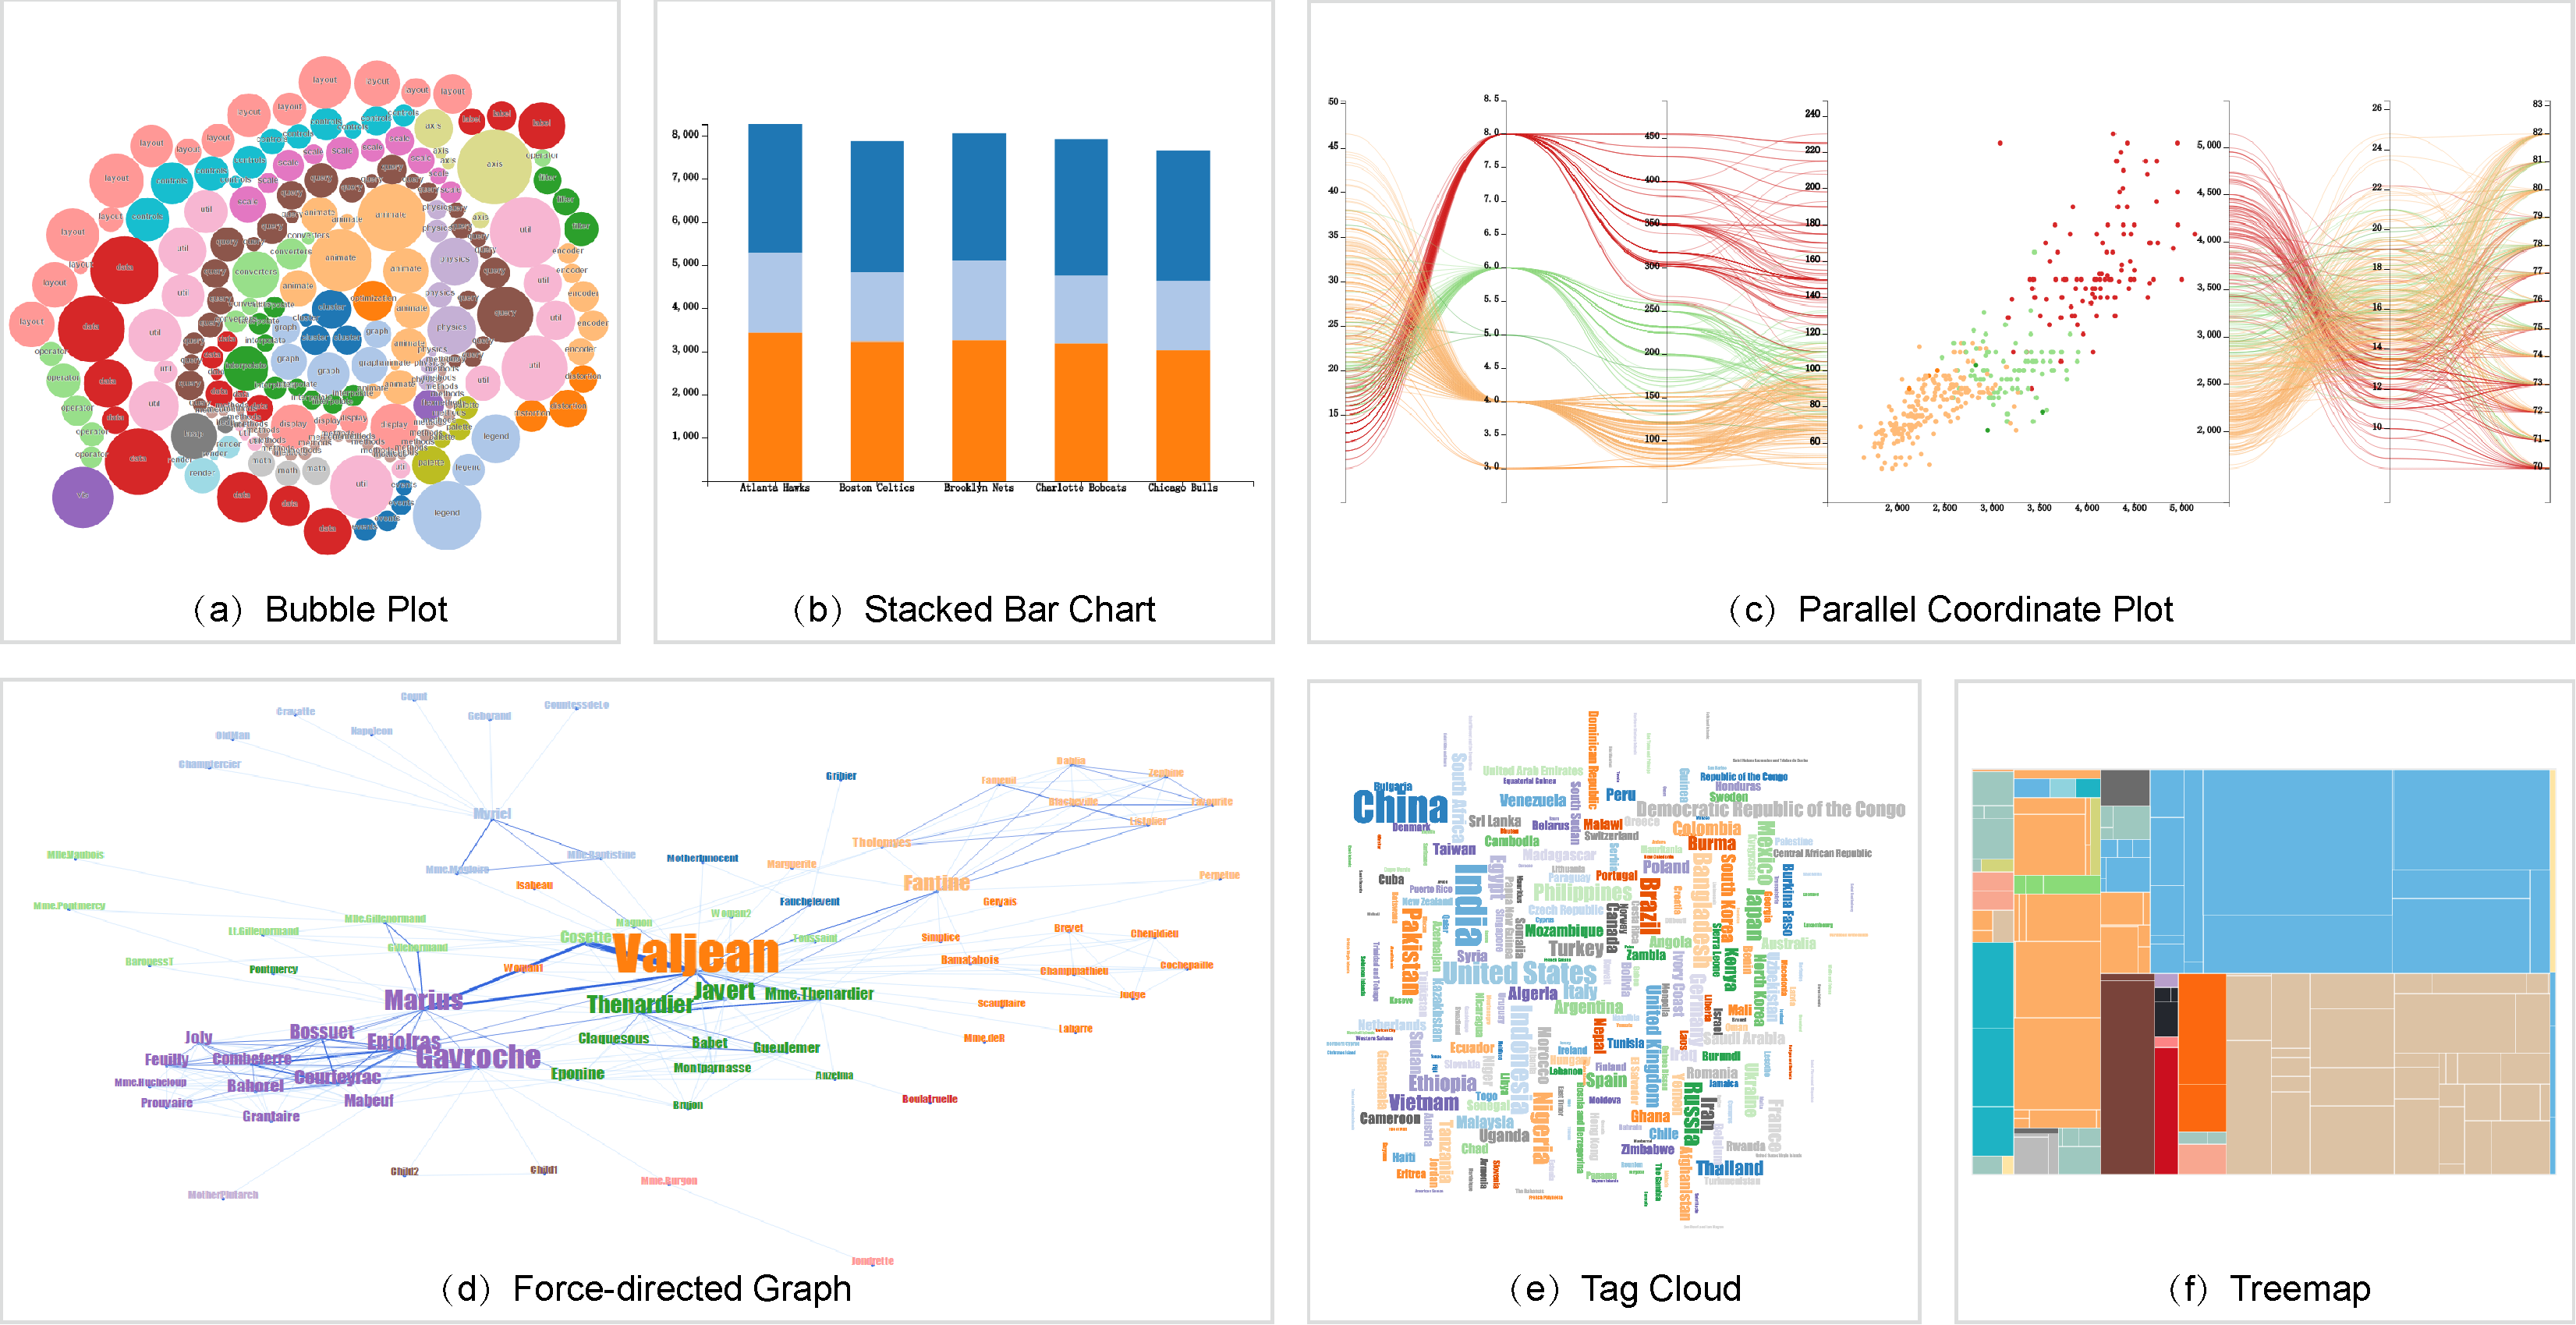
\includegraphics[width=2.0\columnwidth]{images/teaser.pdf}
  \caption{Examples of the visualization designs with VisComposer.}
  \label{teaser}
  }

%% Uncomment below to disable the manuscript note
%\renewcommand{\manuscriptnotetxt}{}

%% Copyright space is enabled by default as required by guidelines.
%% It is disabled by the 'review' option or via the following command:
% \nocopyrightspace

%%%%%%%%%%%%%%%%%%%%%%%%%%%%%%%%%%%%%%%%%%%%%%%%%%%%%%%%%%%%%%%%
%%%%%%%%%%%%%%%%%%%%%% START OF THE PAPER %%%%%%%%%%%%%%%%%%%%%%
%%%%%%%%%%%%%%%%%%%%%%%%%%%%%%%%%%%%%%%%%%%%%%%%%%%%%%%%%%%%%%%%%

\begin{document}
%\begin{CJK*}{GBK}{song}

%% The ``\maketitle'' command must be the first command after the
%% ``\begin{document}'' command. It prepares and prints the title block.

%% the only exception to this rule is the \firstsection command
%\firstsection{Introduction}

\maketitle

%% \section{Introduction} %for journal use above \firstsection{..} instead
\section{Introduction}
\label{sec:intro}
As the amount of data being collected has increased, the need for tools that can enable the visual exploration of data has also grown.  This has led to the development of a variety of widely used programming frameworks for information visualization~\cite{Flare,Processing,Heer:2009:TVCG,Heer:2011:TVCG,Heer:2010:TVCG,Heer:2005:CHI}.  Unfortunately, such frameworks demand comprehensive visualization and coding skills and require users to develop visualization from scratch. As such, these visualization programming toolkits and languages require a large amount of effort for developing appropriate visualization solutions, thereby making visualization nearly intractable for non-programming experts.  Furthermore, conventional programming toolkits or languages seldom integrate with a What You See Is What You Get editor. Thus, they rarely support interactive configurations, thereby stifling collaboration between coders and visual artists in a shared and unified environment.

As such, a recent trend in information visualization is focused on creating interactive visualization design environments that require little to no programming~\cite{Wijk:2011:TVCG,Victor}.  Tools such as Lyra~\cite{Heer:2014:CGF} and iVisDesigner~\cite{Yuan:2014:TVCG} have been created as visualization production tools that allow users to create sophisticated layouts and transformations that are enabled via transformation pipelines.  Unfortunately, these visualization production tools offer support for only a small portion of visual forms, thereby greatly limiting the design space.  As such, expressive visualizations for multivariate and heterogeneous datasets that can easily be created with visualization languages or toolkits like D3~\cite{Heer:2011:TVCG} and Processing~\cite{Processing}, can be difficult to realize in many current visualization production tools.  For instance, Lyra~\cite{Heer:2014:CGF} only operates on tabular datasets, and iVisDesigner~\cite{Yuan:2014:TVCG}, while being very efficient at generating coordinate systems, does not support the construction of recursive drawings such as treemaps.  Furthermore, specifying customized visual designs in these tools is only feasible when the interaction workload is moderate, such as mapping selected data dimensions to appropriate visual channels, or modulating the color scheme for a group of selected data items. The task of managing and customizing detailed designs on a large data set becomes increasingly complicated or even intractable.

Unfortunately, the extremes of a fully programmable solution and a purely interactive non-programmable design environment have major shortcomings. In this paper, we propose a hybrid solution in the form of a novel programmable integrated development environment (IDE), VisComposer.  Such hybrid solutions have a long history in the graphics community.  For example, with the development of shading languages~\cite{RenderMan,OpenGLSL} and programmable graphics hardware, shader-based programs replaced the traditional fixed rendering pipeline to achieve more comprehensive effects~\cite{RTVG,Rieder:2011:CGF}.  To further improve performance and flexibility, many interactive shader development environments, such as RenderMonkey~\cite{RenderMonkey} and FX Composer~\cite{FXComposer}, were created to provide graphic artists with an IDE that served as both a production tool and a programmable interface.

VisComposer has been designed with the goal of making visualization design and optimization easier by providing an intuitive user interface to customize effects with rich authoring controls. Our hybrid solution improves on previous work by enlarging the design space of visualization available to the user.  This is enabled through a custom scene graph in which every component of the visualization process can be configured, edited, and shared.  To facilitate this process, we modularize the visualization design process into components that can be manipulated individually and composed to ensure the efficient, customized, and synchronized production of information visualization. We also adopt the design concepts of shaders from computer graphics in the context of information visualization, where each node in our scene graph can be defined as a piece of program that creates a specific visualization effect. VisComposer  not only provides a drag-and-drop visual editor for rapid prototyping of data-driven visualization, but also enables customization of special effects through textual programming. Our system compares favorably with existing IDEs~\cite{Yuan:2014:TVCG,Heer:2014:CGF} in that it allows for pre-defined visualization creation, while enhancing this through programmable operations, thereby creating a visualization composition language and a visual composer that supports the easy integration of various visualization components, as demonstrated with several examples shown in Figure~\ref{teaser}. Our contributions include:
\begin{itemize}
\item A visualization composition model that modularizes the visualization design process and abstracts the resultant visualization as a scene graph, in which nodes and edges are editable and programmable.
\item A visualization composer that provides a set of operations to enable intuitive and programmable visualization design. Its implementation is built upon the JavaScript language and is compatible with JavaScript-based visualization programs, e.g. D3.js~\cite{Heer:2011:TVCG}.
\item An integrated visual composition environment that empowers users with the ability to directly program visualization effects and immediately view the results of their programming operations.  In this way, we can reduce the time needed for development while still providing the flexibility for novel visualization design.  Such an environment enables the quick iteration of novel designs that cannot be encapsulated in a non-programmable environment.
\end{itemize}






\section{Related Work}
\label{s:relatedwork}

\noindent \textbf{Visualization Programming Frameworks and Languages}
Over the years, a variety of frameworks and languages have been developed with varying degrees of uptake~\cite{Haeberli:1988:SIG,Wilkinson:Grammar}.  The Infovis toolkit~\cite{Fekete:2004:VIS} is an interactive graphics toolkit written in Java that provides a large set of visualization components and supports fast dynamic queries. A distinctive feature of the Infovis toolkit is that it enables many user interactions, e.g. fisheye lenses, dynamic labeling, etc. Improvise~\cite{Weaver:2004:VIS} is another attempt to provide developers with a fully-implemented Java software architecture with a declarative visual query language. It enables users to build and browse highly-coordinated visualizations through a visual interface. The focus of Improvise is on user-driven exploration of complicated datasets across multiple views. Flare~\cite{Flare} is an ActionScript library for creating visualizations that runs in the Adobe Flash Player. It supports data management, visual encoding, animation, and interaction of a list of visual forms. Prefuse~\cite{Heer:2005:CHI} is a software framework for producing dynamic visualizations with structured or unstructured data. The abstractions provided by Prefuse follow the data visualization pipeline proposed in Card et al.~\cite{Card:1999}. Processing~\cite{Processing} is a programming language that was initially designed as a software sketchbook to teach computer programming fundamentals within a visual context. Due to its simplicity, it is widely used by programmers, designers and visual artists. ProtoVis~\cite{Heer:2009:TVCG,Heer:2010:TVCG} is a declarative, domain-specific language for constructing interactive visualizations across platforms. A scenegraph is employed to organize the visual design. D3.js~\cite{Heer:2011:TVCG} inherits the basic abstractions from ProtoVis and improves the browser compatibility by directly binding the input data to standard document object model (DOM).

Each of these frameworks and languages has enabled analysts with varying degrees of expertise to create and share interactive data visualizations.  The power of these languages is in their extendability to create both traditional and novel visualizations.  The ubiquity of visualizations created by these libraries shows that there is a need for these visualization programming languages.  However, researchers have also recognized that there is a large overhead in using these programming languages to create visualizations from scratch.

\noindent \textbf{Integrated Development Environments for Visualization} The need for a faster visualization development time has led to the development of integrated environments for visualization~\cite{Silva:2005:VIS,Lee:2013:TVCG,Myers:1994:CHI}.  Commercial information visualization software and tools, such as Tableau and Manyeyes~\cite{Viegas:2007:TVCG}, provide the user with a drag-and-drop interface for creating visualizations from the scratch. However, the resultant visualization designs are typically adopted from canned visual forms, making it difficult (or in some cases impossible) to create novel customized visualization or effects.

Recent work has sought to improve the user experience and allow for a variety of expressive visualization creations.  For example, Lyra~\cite{Heer:2014:CGF} seeks to improve the expressiveness  by mapping the conventional data visualization  pipeline into a visual editor. The input data is interactively bound to the properties of graphical marks, and the author can design a new visualization which is represented as a specification in Vega~\cite{Vega} which then enables  the sharing and reuse of the visualization product. Similarly, iVisDesigner~\cite{Yuan:2014:TVCG} supports the interactive design of expressive visualization for heterogeneous datasets, covering a broad range of the information visualization design space.
Other tools include Ellipsis~\cite{Heer:2014:Ellipsis}, which implements a model of storytelling abstractions and a domain-specific language (DSL)  within a graphical interface for effective story authoring.

While these systems advance previous solutions by enabling visualization customization without writing code, the design space available to the visualization authors is still limited. On the other hand, the language based approach of building each visualization from scratch also has considerable drawbacks.  As such, it seems natural to integrate programming capability within an IDE for Visualization.  VisComposer presents a hybrid solution combining options for programmability into an IDE for visualization.  By enabling users to directly add code segments for customizable and extensible visualizations, our work is able to reduce the programming overhead common among visualization languages while still providing much of their flexibility.


One main advantage of integrating programmability into the graphical development environments is its flexibility and expressiveness. For example, in computer graphics and scientific visualization, shader programs~\cite{RTVG,OpenGLSL} are typically written to apply transformations to a large set of elements, e.g., to each pixel in a window. This is very suitable for parallel processing, and most GPUs have multiple shader pipelines to facilitate this parallelism, vastly improving computation throughput. Our approach shares the same benefit in that a visualization operation written within the interactive visualization environment can be applied to many data points, avoiding individual specifications of the intended operations.

\input{design.tex}
\input{language.tex}
\input{composer.tex}
\section{Interactive Visualization Design Environment}
\label{sec:environment}
In this section, we will describe our web-based visualization design environment, VisComposer.

\subsection{The Interface}
The interface (Figure~\ref{fg:interface}) contains four main views corresponding to four modules of the visualization composition model. All widgets and views are designed to be collapsible so that more
screen space can be preserved for the main view.

The \textbf{resource} view~(Figure~\ref{fg:interface} (a)) shows the resources being used in designing visualizations. The view contains four main components that list the names, structures and properties of data and the data primitives, composition operators and visual forms. Detailed information of selected items (e.g., the input dataset) can be further explored using additional popup windows. Our system supports the loading and composition of multiple datasets and visual forms.

The \textbf{visualization} view (Figure~\ref{fg:interface} (b)) is the container of the visualization being designed.  It is updated whenever a modification is made during the design process. To enable quick design iterations, the view is synchronized with the creation of the scenegraph.  A proxy geometry or graphical glyph is shown if a node or link of the underlying scenegraph has not been bound, or if a primitive has not been mapped to a visual propertiy. Interactive specification and manipulation of the graphical primitives or forms in the view is allowed.

The \textbf{scenegraph} view (Figure~\ref{fg:interface} (c)) shows the scenegraph structure of the visualization and enables many user interactions that represent the abstract and interact operations defined in Section 5.1. The user can create nodes, links and compose the visualization within this view. The tree shows the basic information of each node and link, such as the type of primitives, the underlying data selectors and the composition operators. The user can edit nodes and links interactively or load from stored forms as a prototype template.

The \textbf{transformation} view is the workbench for performing the bind, map and abstract operations. A suite of textual and configuration panels (Figure~\ref{fg:interface} (d)) are provided for user modulations. The user can craft transformations by editing ones provided by the system or write a visualization shader.

\begin{figure*}
  \centering
  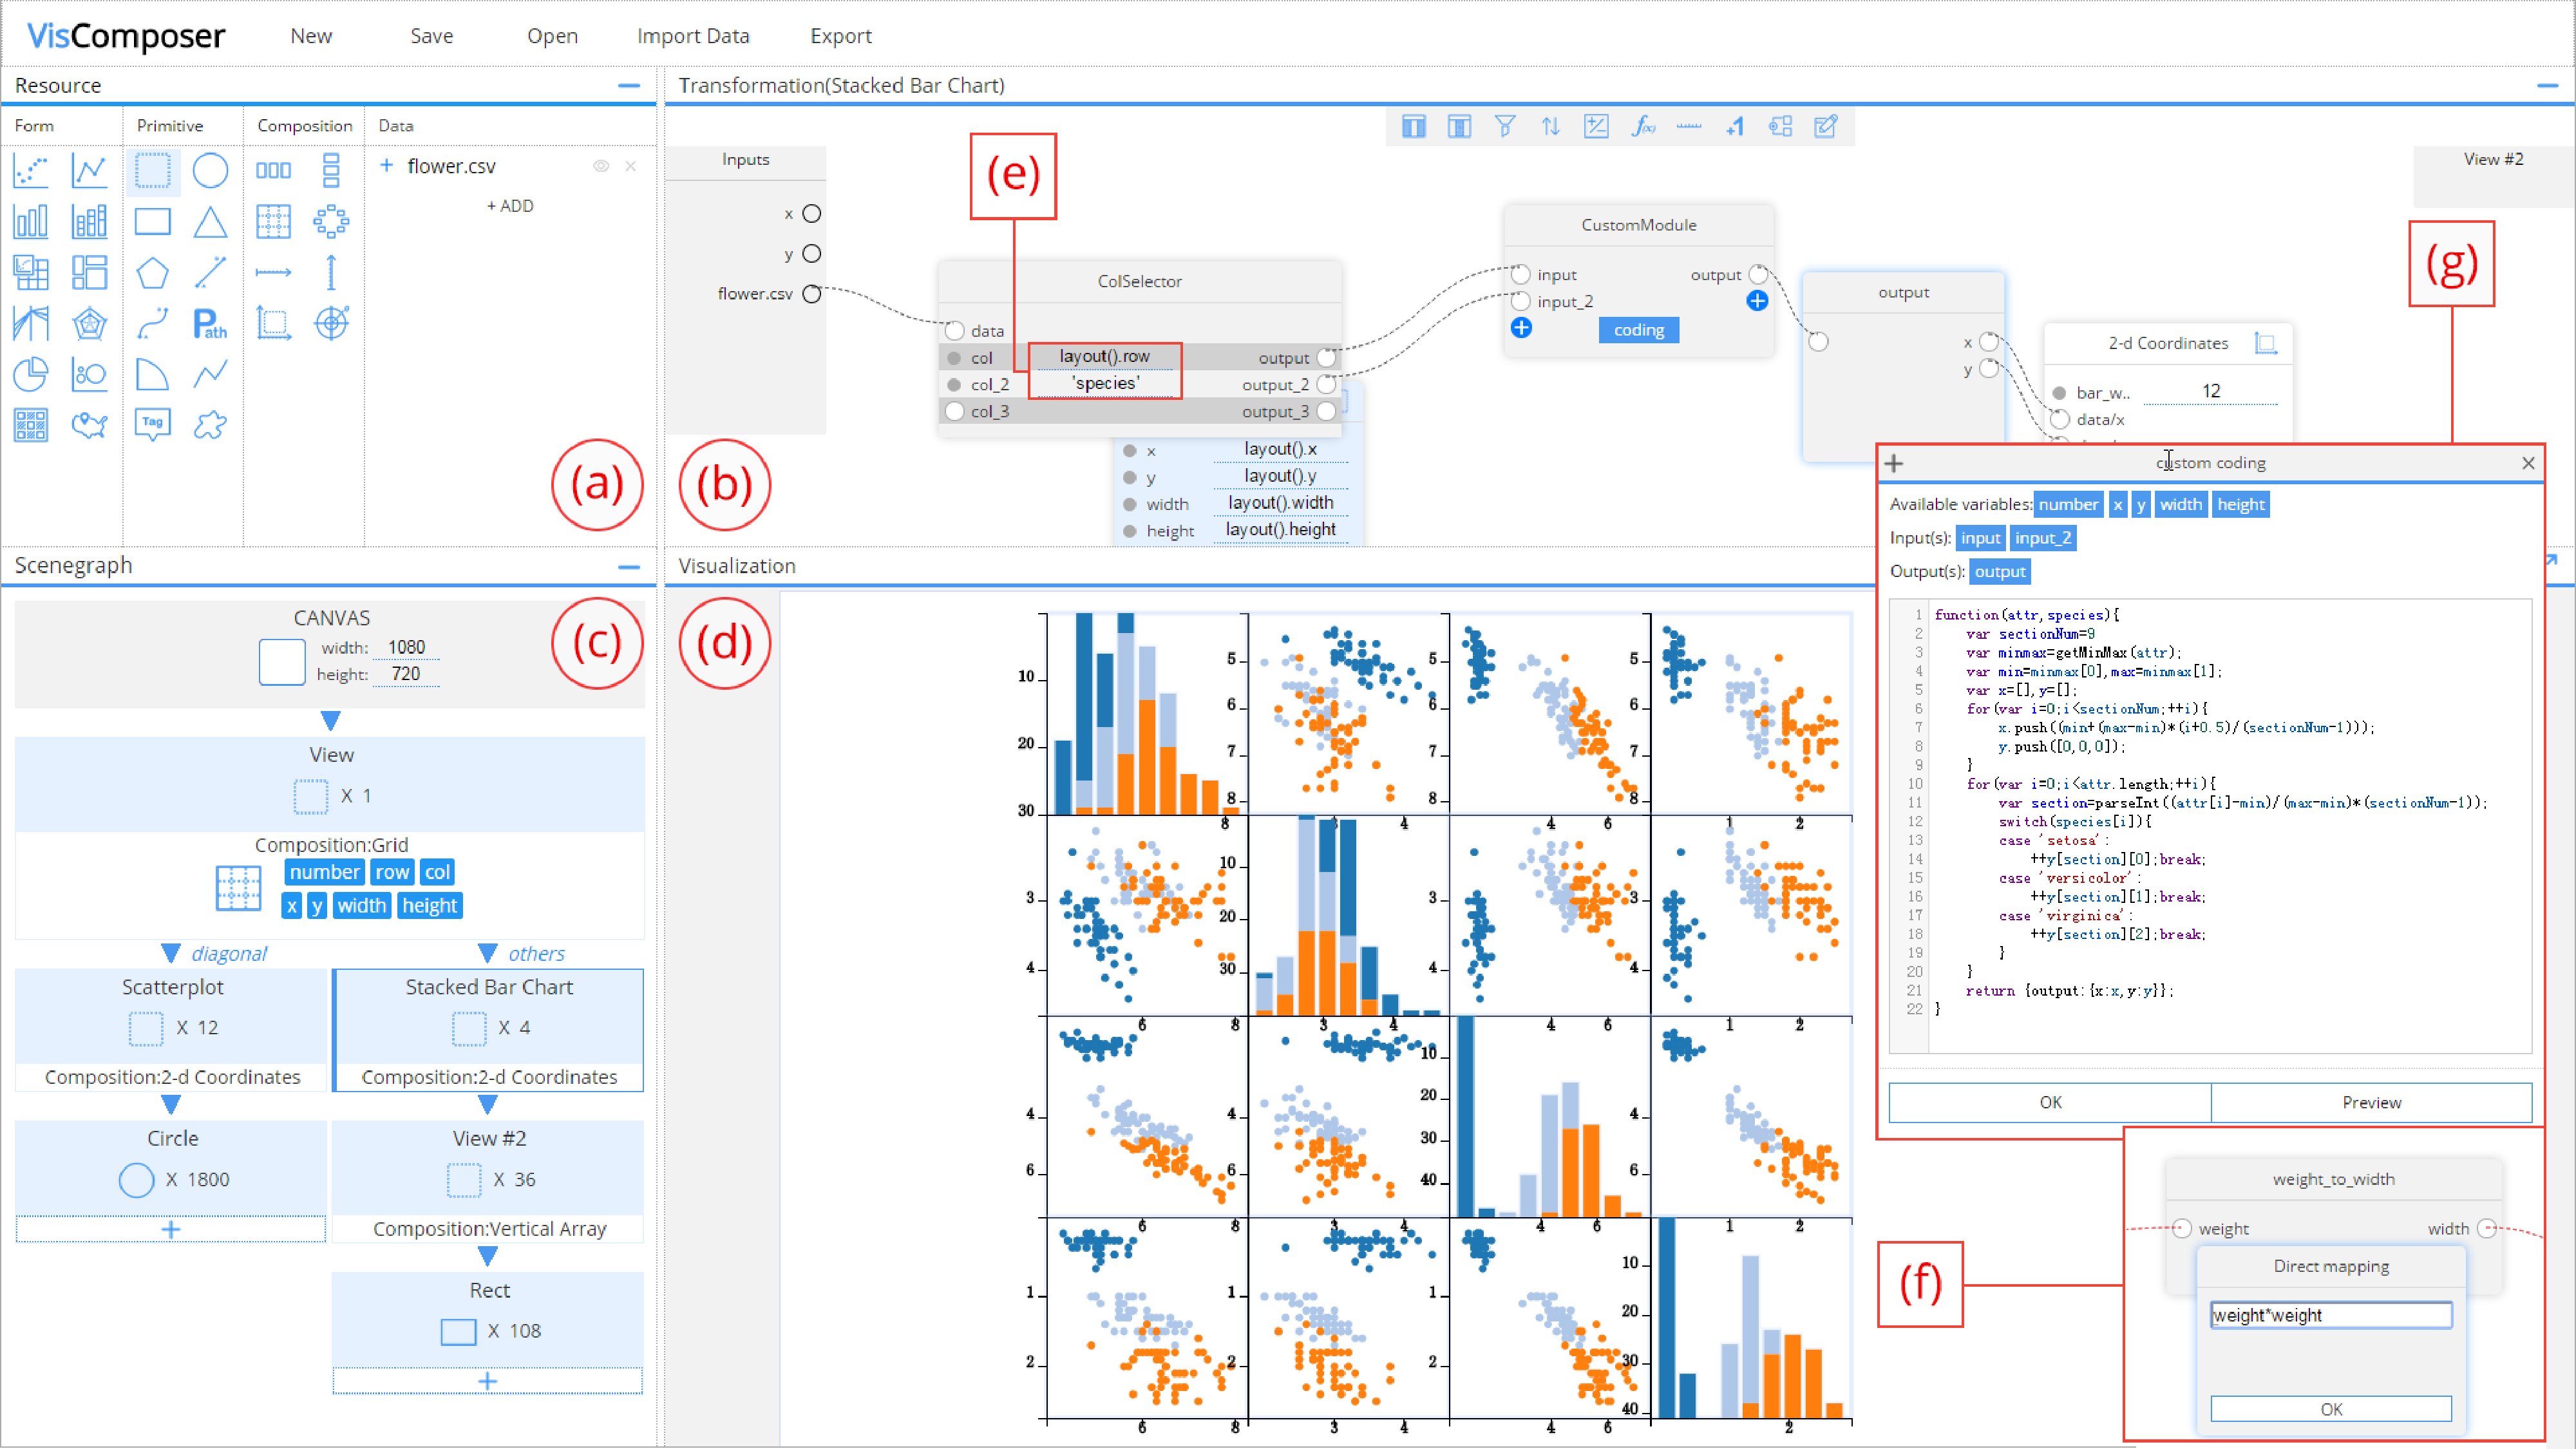
\includegraphics[width=0.98\linewidth]{images/system.pdf}
  \caption{The interface of VisComposer: (a) the resource view, (b) the transformation view, (c) the scenegraph view, and (d) the visualization view. \newline(e) $\scriptsize{\sim}$ (h) Editors for the three types of programmable shaders.
  %and (e) the code editor window of a custom transformation. 
  The scatterplot matrix representation of Iris Flower Dataset is displayed.}
  \label{fg:interface}
\end{figure*}

\subsection{User Interactions}
To compose a visualization, the user can perform operations of the visualization composition model by interactively manipulating data, primitives, composition operators, visual forms, and intermediate structures, such as the scenegraph.  The composition process begins only after a dataset is loaded.  User interactions with the VisComposer interface can be defined as follows.

\noindent \textbf{Selection}: Two types of selection tools are provided to facilitate the specification of points of interest. The lasso selection tool supports brushing a rectangular or an arbitrary shaped region within the visualization or transformation view to select data items or primitives directly. Alternatively, the user can select the data items or primitives by double clicking on the nodes or links in the scenegraph view.

\noindent \textbf{Drag-and-drop}: To transfer selected items in or across different views, the user can drag the object from the original view to the destination.

\noindent \textbf{Painting}: The user can freely draw an axis or other geometry in the visualization canvas in order to directly specify the visual design. The paint tools can help the user quickly specify properties of a new visual structure and refine them if needed. A set of docking points are utilized for the purposes of positioning and designing composition modes.

\noindent \textbf{Programming}: In the transformation view and the scenegraph view most of the elements are programmable. The user can bind data by using a short expression in an input box, or create a functional modifier to assign a custom visual mapping. The user can also trigger a code editor and write scripts in JavaScript. Quick debugging of code is enabled by the interactive output of intermediate results in the visualization view. The user can view the programmed effects by examining individual operations in the visualization view.

\noindent \textbf{Annotations}: The user can identify and analyze the results through free-style annotations. Iconic and textual annotations are supported.

\subsection{Two Design Modes}
VisComposer enables both high-level and low-level control features for use by technical developers as well as purely visual controls to enable visualization design by non-technical artists. Two design modes are provided: design from scratch or template-based design.

\noindent \textbf{Design from scratch:} This mode requires the user to build elements from scratch. Generally, the user follows the flowchart depicted in Figure~\ref{fg:flowchart} to craft a visualization. For modification, the user can flexibly erase, restore, and restart an ongoing composition by means of the interface. Any element can be edited by either programming or pre-defined interactions if necessary.

\noindent \textbf{Template-based design} To simplify the customization of effect and share visualization, a high-level manipulation mode is supported by leveraging the visual forms. By default, a visual form can be formulated based on a template representation. When a template is selected or loaded, the environment automatically instantiates the scenegraph structure. All the components in a template are editable and programmable. In this way, the user can bypass the tedious setup steps and dive straightly into the visualization design process.

\subsection{The Implementation Details}
%The implementation of VisComposer is based on HTML5 with jQuery.

\indent \textbf{Data Format:} VisComposer stores and manipulates data as JavaScript Objects. Data sources, such as CSVs, JSONs, can be loaded and converted to objects. VisComposer provides a flexible data type control to improve data import. Profiles of the input data, such as the data types and dimensions, are kept and can be used in the composition process.
%User-defined data could benefit from it by auto detecting or explicitly declaring.

\noindent \textbf{Drawing:} VisComposer outputs a structured representation of primitives.  Then these primitives are sent to the renderer  in a batch mode. In general, there are two modes for rendering the primitives: creating and displaying SVG nodes which support mouse and keyboard interaction from the browser; drawing in the canvas to generate a static result. To support interactive development, VisComposer utilizes the SVG mode during the visualization composition process. Exporting the result in to HTML5 canvas is also supported when publishing the design.
%and then allows for drawing in the canvas when the design is completed.

\noindent \textbf{Interaction:} VisComposer provides rich user controls which are synchronized among different views. For example, moving an element in the visualization view leads to the changes of its \emph{x} and \emph{y} coordinates in the Transformation view; creating a visual mapping in the transformation view modifies the  scenegraph and the visualization.
%Essentially, the user interaction mode mirrors the code writing mode.
In this way, the user can quickly compose a visualization with user-friendly interactions and obtain real-time feedback in the visualization module.
%customize through scripting.

\noindent \textbf{Serialization:} A visualization is composed of a list of JavaScript objects that are referenced to each other. Similar to iVisdesigner~\cite{Yuan:2014:TVCG}, VisComposer serializes all objects and maintains references to enable external storage, loading and reuse of components. VisComposer assigns a universally unique identifier (UUID) to each object that represents references out of memory. The  object collection of a visualization is processed in depth-first order and objects are stored when they first occur. Specifically, we employ an enhanced serialization scheme that the user can only save part of the pipelines or a sub-tree of the scenegraph into an offline file. Other users can import the file to re-use the component as part of the current design.
%A hashmap using UUIDs as keys is built to guarantee objects are stored as references. When there are more than one reference, the keys can be used to restore the structure. Moreover, an identifier which records the object type is stored and refers to the right constructor to be called while restoring.

\noindent \textbf{Reuse and Export:} VisComposer supports the reuse and exportation of visualizations in three ways: 1) The designed visualization can be exported as a bitmap image or vector graph; 2) The workspace can be exported and saved as a template file for future reuse; 3) The design can be packed with a runtime library,  which can be embedded into an HTML page. 
\input{examples.tex}
\input{evaluations.tex}
\section{Conclusions}
\label{sec:con}
This paper presents a visual authoring environment that enhances the conventional visualization pipeline with an abstractive design structure and programmable scheme. The contribution is a novel visual programmable design scheme that visually represents the modularized visualization pipeline and allows for an interactive management and composition of the visualization process. The implemented system not only allows easy visualization design and development, but also provides a mechanism for managing the designs of the associated visual resources in a single environment. One of its distinctive features is its inclusion of textual programming to support the programmable development of novel visualization effects. The interactivity of the program enables fast content development, quick design iteration, and customizable effects. Finally, the results made with our system can be easily integrated into the workflow of other visualization programs.


%% if specified like this the section will be committed in review mode
%\acknowledgments{
%The authors wish to thank A, B, C. This work was supported in part by
%a grant from XYZ.}

\bibliographystyle{abbrv}
%%use following if all content of bibtex file should be shown
%\nocite{*}
\bibliography{template}
%\end{CJK*}
\end{document}
